\documentclass[pdftex]{article}
\usepackage[dvips]{graphicx} 
\usepackage{pslatex}	
\usepackage{floatrow}
\usepackage{url}
\usepackage{amsmath}
\usepackage{hyperref}
\title{Arya Sikder}
\author{CH22B006}
\date{Aryeahh}
\begin{document}
\maketitle
\section{Introduction}
The \textit{Redlich-Kwong}\footnotemark[1] equation helps us calculate \textbf{state of an real gas} as with much better accuracy than \textit{van der Waal's} equation at temperatures \textbf{above the critical temperature.}\footnotemark[2]  It is largely an emperical formula.
\section{The Equation}
\begin{center}
    \boxed{$${\displaystyle p={\frac {R\,T}{V_{m}-b}}-{\frac {a}{{\sqrt {T}}\;V_{m}\,(V_{m}+b)}},}$$ }
\end{center}
\begin{itemize}
    \item[--] \textbf{p}, \textbf{T}, \textbf{$V_m$} : gas pressure, temperature, molar volume
    \item[--] \textbf{R} : universal gas constant
    \item[--] \textbf{a} : constant arising due to interaction potential between gas molecules
    \item [--] \textbf{b} : constant arising due to space taken up by molecules
\end{itemize}

\begin{figure}[h]
    \centering
    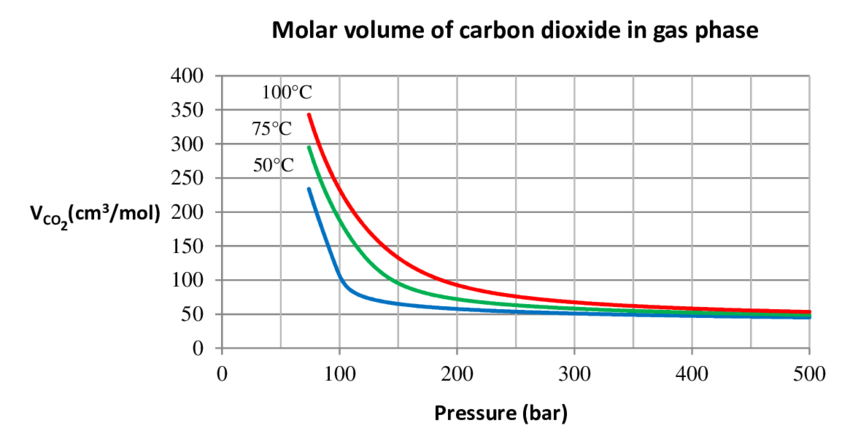
\includegraphics[scale = 0.8]{Redlich-Kwong equation.png}
    {\caption{P vs $V_m$ for $CO_2$ at different temperatures}\label{fig:}}
\end{figure}

\footnote[1]
{\href{https://chem.libretexts.org/Courses/Colorado\_State\_University/Chem\_476\%3A\_Physical\_Chemistry\_II\_(Levinger)/Chapters/16\%3A\_The\_Properties\_of\_Gases/16.2\%3A\_van\_der\_Waals\_and\_Redlich-Kwong\_Equations}{Redlich-Kwong equation}}
\footnote[2]
{\href{https://chem.libretexts.org/Bookshelves/General\_Chemistry/Book\%3A\_General\_Chemistry\%3A\_Principles\_Patterns\_and\_Applications\_(Averill)/11\%3A\_Fluids/11.06\%3A\_Critical\_Temperature\_and\_Pressure}{Critical Temperature}}



\end{document}
